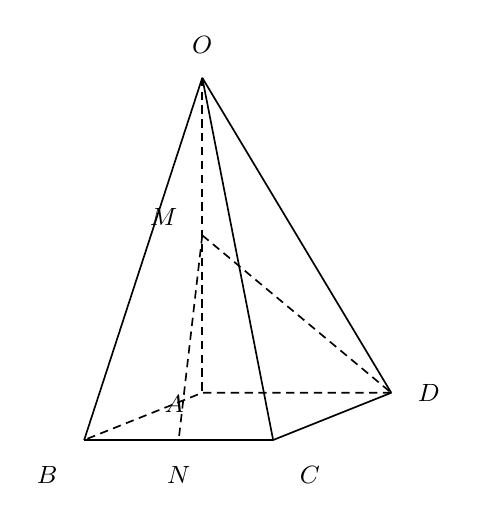
\begin{tikzpicture}[line width=0.6pt, font=\small]
\coordinate (A) at (0,0.6);
\coordinate (B) at (-1.5,0);
\coordinate (C) at (0.9,0);
\coordinate (D) at (2.4000000000,0.6000000000);
\coordinate (O) at (0.0000000000,4.6000000000);
\coordinate (M) at (0.0000000000,2.6000000000);
\coordinate (N) at (-0.3,0);
% base
\draw[solid] (B) -- (N) -- (C) -- (D);
\draw[densely dashed] (D) -- (A) -- (B);
% height and laterals
\draw[densely dashed] (O) -- (A);
\draw[solid] (O) -- (B);
\draw[solid] (O) -- (C);
\draw[solid] (O)--(D);
% auxiliary segments from M
\draw[densely dashed] (M) -- (D);
\draw[densely dashed] (M) -- (N);
\node[above=5pt] at (O) {$O$};
\node[left=7pt,above=3pt,xshift=-7pt,yshift=-3pt] at (M) {$M$};
\node[below=7pt,left=2pt,xshift=-1pt,yshift=3pt] at (A) {$A$};
\node[below left=6pt] at (B) {$B$};
\node[below=6pt] at (N) {$N$};
\node[below right=6pt] at (C) {$C$};
\node[right=6pt] at (D) {$D$};
\end{tikzpicture}
